\documentclass[11pt,a4paper]{article}

\usepackage[utf8]{inputenc}
\usepackage[T1]{fontenc}
\usepackage[margin=2.5cm]{geometry}
\usepackage{amsmath,amssymb,amsthm}
\usepackage{booktabs}
\usepackage{enumitem}
\usepackage{xcolor}
\usepackage{tikz}
\usepackage{hyperref}

\newtheorem{theorem}{Theorem}
\newtheorem{lemma}[theorem]{Lemma}
\newtheorem{corollary}[theorem]{Corollary}
\theoremstyle{definition}
\newtheorem{definition}[theorem]{Definition}
\newtheorem{example}[theorem]{Example}
\theoremstyle{remark}
\newtheorem{remark}[theorem]{Remark}

\newcommand{\lex}{\preceq}
\newcommand{\slex}{\prec}
\newcommand{\nb}{N}
\newcommand{\Lst}{L}
\newcommand{\red}[2]{\mathrel{\preceq_{#1#2}}}
\newcommand{\sred}[2]{\mathrel{\prec_{#1#2}}}

\tikzset{
  vtx/.style={circle,draw,thick,minimum size=6mm,inner sep=0pt,font=\small},
  gedge/.style={thick}
}

\title{Decreasing Lexicographic Order on Neighbor Lists:\\
a Sound Symmetry-Breaking Constraint for Graph Enumeration}
\author{}
\date{}

\begin{document}
\maketitle

\begin{abstract}
In the \emph{neighbors model} a graph on $n$ vertices is represented by $n$ neighbor
lists of length $n-1$, padded with leading zeros. We prove that requiring these lists to be
\emph{lexicographically non-increasing}, $\Lst(1)\succeq \Lst(2)\succeq\dots\succeq \Lst(n)$,
is a \emph{sound} symmetry-breaking constraint: every graph has at least one labelling that
satisfies it. The proof translates the order on lists into an order on the rows of the
adjacency matrix (Lemma~\ref{lem:bridge}) and then reuses the vertex-swap argument of
Codish, Miller, Prosser and Stuckey~\cite{codish13,codish19}, restricted to labellings
with non-increasing degrees. We also show, with the one-edge graph $K_2$ as a counterexample, why the \emph{increasing}
order is not sound, and
that the decreasing order is incompatible with the upper off-diagonal connectivity constraint.
\end{abstract}

%=====================================================================
\section{Setting and notation}
%=====================================================================

Let $G=(V,E)$ be a simple undirected graph with $V=\{1,\dots,n\}$, $n\ge 2$.

\begin{definition}[Adjacency rows]
$A\in\{0,1\}^{n\times n}$ is the adjacency matrix of $G$: $A[u][v]=1$ iff $\{u,v\}\in E$.
It is symmetric and $A[v][v]=0$ (no self-loops). The \emph{row} of $v$ is the vector
$A[v]=(A[v][1],\dots,A[v][n])$. We write $\deg(v)=\sum_w A[v][w]$ and
$\nb(v)=\{w : A[v][w]=1\}$.
\end{definition}

\begin{definition}[Lexicographic order]
For two sequences $x,y$ of equal length, $x\slex y$ iff at the first position $k$ where they
differ, $x_k<y_k$; and $x\lex y$ iff $x\slex y$ or $x=y$. Positions are read left to right.
\end{definition}

\begin{definition}[Padded neighbor list]\label{def:list}
The \emph{neighbor list} of $v$ is the sequence of length $n-1$
\[
  \Lst(v)=\bigl(\underbrace{0,\dots,0}_{n-1-\deg(v)},\; w_1,\, w_2,\,\dots,\, w_{\deg(v)}\bigr),
  \qquad \nb(v)=\{w_1<w_2<\dots<w_{\deg(v)}\}.
\]
Empty slots hold $0$ and come first; the neighbors follow in strictly increasing order.
This is exactly the row \texttt{M[v]} of the neighbors model (\texttt{buildBaseModelNei}).
\end{definition}

\begin{definition}[Reduced row comparison, \cite{codish13}]
For $i\neq j$, write $A[i]\red ij A[j]$ when $A[i]\lex A[j]$ after deleting columns $i$ and $j$
from both rows, and $A[i]\sred ij A[j]$ for the strict version.
This is the comparison used by the OptLex constraint.
\end{definition}

\begin{definition}[Upper-triangle string]
$s(A)=\bigl(A[1][2],\dots,A[1][n],\;A[2][3],\dots,A[2][n],\;\dots,\;A[n-1][n]\bigr)$,
the strict upper triangle of $A$ read row by row.
\end{definition}

\begin{definition}[Relabelling]
For a permutation $\pi$ of $V$, $G^\pi$ is the graph in which vertex $v$ of $G$ receives label
$\pi(v)$; its adjacency matrix satisfies $A^\pi[\pi(u)][\pi(v)]=A[u][v]$. Graphs related by
a relabelling are \emph{isomorphic}; an isomorphism class is called a \emph{shape}.
\end{definition}

\begin{definition}[Soundness]
A constraint $C$ on labelled graphs is \emph{sound} if every graph has at least one
relabelling satisfying $C$, i.e.\ no shape is lost. It is \emph{complete} if exactly one
labelling per shape satisfies it.
\end{definition}

\begin{definition}[The two orders on neighbor lists]
\begin{align*}
  \textsc{Dec}(G):&\quad \Lst(1)\succeq \Lst(2)\succeq\dots\succeq \Lst(n)
    &&\text{(non-increasing lists)},\\
  \textsc{Inc}(G):&\quad \Lst(1)\lex \Lst(2)\lex\dots\lex \Lst(n)
    &&\text{(non-decreasing lists)}.
\end{align*}
\end{definition}

The main result is:

\begin{theorem}[Main theorem]\label{thm:main}
\textsc{Dec} is sound: every graph $G$ has a relabelling $G^\pi$ whose padded neighbor
lists are lexicographically non-increasing. The same holds when every vertex is required
to have the same degree $d$ ($d$-regular graphs).
\end{theorem}

\textsc{Inc}, in contrast, is \emph{not} sound (Section~\ref{sec:inc}).

%=====================================================================
\section{From neighbor lists to adjacency rows}
%=====================================================================

\begin{lemma}[Bridge lemma]\label{lem:bridge}
Let $u,v$ be two vertices.
\begin{enumerate}[label=(\alph*)]
  \item If $\deg(u)>\deg(v)$ then $\Lst(u)\succ \Lst(v)$.
  \item If $\deg(u)=\deg(v)$ then
  \[
     \Lst(u)\succeq \Lst(v) \iff A[u]\lex A[v].
  \]
\end{enumerate}
So the list order compares the degree first and, for equal degrees, it is the
\emph{reverse} of the order on the 0/1 adjacency rows.
\end{lemma}

\begin{proof}
(a) Let $p=n-1-\deg(u)$ be the number of leading zeros of $\Lst(u)$; $\Lst(v)$ has
$n-1-\deg(v)>p$ leading zeros. Positions $1,\dots,p$ are $0$ in both lists, and at position
$p+1$ the list $\Lst(u)$ holds a neighbor (a label $\ge 1$) while $\Lst(v)$ still holds $0$.
Hence $\Lst(u)\succ\Lst(v)$.

(b) Both lists have the same number of leading zeros, so they can only differ in their
neighbor parts $(a_1<\dots<a_t)$ for $u$ and $(b_1<\dots<b_t)$ for $v$, with $t=\deg(u)$.
If $\nb(u)=\nb(v)$ then $\Lst(u)=\Lst(v)$ and $A[u]=A[v]$, and both sides hold.
Otherwise let $k$ be the first index with $a_k\ne b_k$, so $a_r=b_r$ for $r<k$.

Suppose $a_k>b_k$, i.e.\ $\Lst(u)\succ\Lst(v)$. The label $b_k$ belongs to $\nb(v)$.
It does not belong to $\nb(u)$: the elements of $\nb(u)$ smaller than $a_k$ are exactly
$a_1,\dots,a_{k-1}=b_1,\dots,b_{k-1}$, all smaller than $b_k$. Every label $w<b_k$ is either
one of the common elements $b_1,\dots,b_{k-1}$ or in neither set. Therefore column $b_k$ is the
first column where the rows $A[u]$ and $A[v]$ differ, with $A[u][b_k]=0<1=A[v][b_k]$, that is
$A[u]\slex A[v]$.

Symmetrically, $a_k<b_k$ gives $A[u]\succ A[v]$. Since exactly one of the two cases occurs
when the lists differ, $\Lst(u)\succ\Lst(v)\iff A[u]\slex A[v]$, which together with the case
of equality proves (b).
\end{proof}

\begin{corollary}[\textsc{Dec} in adjacency terms]\label{cor:dec}
$G$ satisfies \textsc{Dec} if and only if for all $i<j$:
\[
  \deg(i)>\deg(j)
  \qquad\text{or}\qquad
  \bigl(\deg(i)=\deg(j)\ \text{and}\ A[i]\lex A[j]\bigr).
\]
That is: degrees are non-increasing, and inside each group of equal degree the full adjacency
rows are non-decreasing.
\end{corollary}

\begin{proof}
By transitivity of $\succeq$, $\textsc{Dec}$ is equivalent to $\Lst(i)\succeq\Lst(j)$ for all
$i<j$. By Lemma~\ref{lem:bridge}(a), $\Lst(i)\succeq\Lst(j)$ forces $\deg(i)\ge\deg(j)$; if
$\deg(i)>\deg(j)$ it always holds, and if the degrees are equal it is equivalent to
$A[i]\lex A[j]$ by Lemma~\ref{lem:bridge}(b).
\end{proof}

%=====================================================================
\section{Two lemmas on adjacency rows}
%=====================================================================

\begin{lemma}[Reduced order implies full order]\label{lem:reduced}
Let $i<j$. If $A[i]\red ij A[j]$ then $A[i]\lex A[j]$.
\end{lemma}

\begin{proof}
Let $e=A[i][j]=A[j][i]$. On the full rows, column $i$ reads $(A[i][i],A[j][i])=(0,e)$ and
column $j$ reads $(A[i][j],A[j][j])=(e,0)$. All other columns are those of the reduced rows,
and columns $1,\dots,i-1$ come before both $i$ and $j$.
\begin{description}[leftmargin=1.5em]
  \item[Case 1:] the reduced rows differ at some column $k<i$. The full rows first differ at
  the same column, with the same outcome, so $A[i]\slex A[j]$.
  \item[Case 2:] no difference before column $i$, and $e=1$. Column $i$ of the full rows reads
  $(0,1)$, so $A[i]\slex A[j]$ whatever comes after.
  \item[Case 3:] no difference before column $i$, and $e=0$. Columns $i$ and $j$ both read
  $(0,0)$, so the full comparison equals the reduced one and $A[i]\lex A[j]$.\qedhere
\end{description}
\end{proof}

\begin{remark}\label{rem:diag}
Case~2 is where the zero diagonal enters: if $i$ and $j$ are adjacent, the entry
$A[i][i]=0$ sits to the left of $A[j][i]=1$ and makes row $i$ smaller. This works
\emph{for} a non-decreasing order on rows, and therefore \emph{for} \textsc{Dec}; it works
\emph{against} the opposite order. This is the precise reason for the asymmetry between
\textsc{Dec} and \textsc{Inc} (Section~\ref{sec:inc}).
\end{remark}

\begin{lemma}[Swap lemma, \cite{codish13}]\label{lem:swap}
Let $i<j$ with $A[j]\sred ij A[i]$ (the reduced order of rows $i,j$ is violated), i.e.\
the first column $k\notin\{i,j\}$ where the rows differ has $A[i][k]=1$ and $A[j][k]=0$. Let $\tau$ be the transposition of $i$ and $j$ and
$A'=A^{\tau}$. Then $s(A')\slex s(A)$.
\end{lemma}

\begin{proof}
$A'[x][y]=A[\tau(x)][\tau(y)]$, so only entries in rows or columns $i$ and $j$ change, and
$A'[i][j]=A[j][i]=A[i][j]$. By the choice of $k$, $A[i][x]=A[j][x]$ for every
$x<k$ with $x\notin\{i,j\}$.

\emph{Case $k<i$.} For a row $x<k$ the only entries of $s$ that can change are
$(x,i)$ and $(x,j)$, and $A'[x][i]=A[x][j]=A[j][x]=A[i][x]=A[x][i]$ (similarly for $(x,j)$):
they do not change. In row $k$ the entries $(k,y)$ with $k<y<i$ do not involve $i$ or $j$;
the first entry that may change is $(k,i)$, and
\[
  A'[k][i]=A[k][j]=A[j][k]=0 \quad<\quad 1=A[i][k]=A[k][i].
\]
\emph{Case $k>i$.} Rows $x<i$ are unchanged as above (every such $x$ is smaller than $k$).
In row $i$, $A'[i][y]=A[j][y]$ for $y\neq j$, and $A'[i][j]=A[i][j]$. For $i<y<k$, $y\neq j$,
$A[j][y]=A[i][y]$, so the first entry of row $i$ that changes is $(i,k)$:
\[
  A'[i][k]=A[j][k]=0 \quad<\quad 1=A[i][k].
\]
In both cases the first difference between $s(A')$ and $s(A)$ goes from $1$ to $0$.
\end{proof}

%=====================================================================
\section{Proof of the main theorem}
%=====================================================================

\begin{proof}[Proof of Theorem~\ref{thm:main}]
Let $\mathcal{P}$ be the set of relabellings of $G$ whose degrees are non-increasing,
$\deg(1)\ge\deg(2)\ge\dots\ge\deg(n)$. $\mathcal{P}\neq\emptyset$: sort the vertices by
degree. Choose $G^\ast\in\mathcal{P}$ with adjacency matrix $A$ such that $s(A)$ is
lexicographically \emph{smallest} in $\mathcal{P}$.

Let $i<j$ with $\deg(i)=\deg(j)$, and suppose $A[j]\sred ij A[i]$. Swapping $i$ and $j$
keeps the degree sequence non-increasing (the two degrees are equal), so
$A^\tau\in\mathcal{P}$, and by Lemma~\ref{lem:swap} $s(A^\tau)\slex s(A)$ --- a contradiction
with the choice of $G^\ast$. Hence $A[i]\red ij A[j]$, and by Lemma~\ref{lem:reduced}
$A[i]\lex A[j]$.

So in $G^\ast$: degrees are non-increasing, and inside each group of equal degree the full
rows are non-decreasing. By Corollary~\ref{cor:dec}, $G^\ast$ satisfies \textsc{Dec}.

For $d$-regular graphs all degrees equal $d$, $\mathcal{P}$ contains every relabelling,
and the same argument applies; relabelling never changes degrees, so $G^\ast$ is still
$d$-regular.
\end{proof}

\begin{remark}[What the proof does \emph{not} give]
\textsc{Dec} is sound, not complete: several labellings of the same shape may satisfy it
(Section~\ref{sec:exp}). The canonical labelling $G^\ast$ is only used to prove existence;
the solver is not required to find it.
\end{remark}

%=====================================================================
\section{A worked example}
%=====================================================================

\begin{example}[The path $P_4$]
$P_4$ has two inner vertices of degree $2$ and two leaves of degree $1$. In $\mathcal{P}$ the
inner vertices are $1,2$ (adjacent) and the leaves are $3,4$. Two labellings remain
(with $n-1=3$ slots per list):

\begin{center}
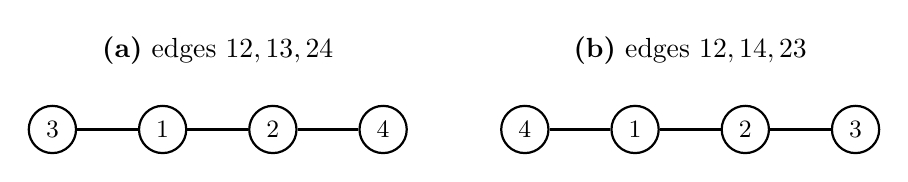
\begin{tikzpicture}[x=1.4cm]
  \node at (1.5,1) {\textbf{(a)} edges $12,13,24$};
  \node[vtx] (a3) at (0,0) {3};
  \node[vtx] (a1) at (1,0) {1};
  \node[vtx] (a2) at (2,0) {2};
  \node[vtx] (a4) at (3,0) {4};
  \draw[gedge] (a3)--(a1)--(a2)--(a4);
  \begin{scope}[xshift=6cm]
  \node at (1.5,1) {\textbf{(b)} edges $12,14,23$};
  \node[vtx] (b4) at (0,0) {4};
  \node[vtx] (b1) at (1,0) {1};
  \node[vtx] (b2) at (2,0) {2};
  \node[vtx] (b3) at (3,0) {3};
  \draw[gedge] (b4)--(b1)--(b2)--(b3);
  \end{scope}
\end{tikzpicture}
\end{center}

\begin{center}
\begin{tabular}{c ccc c ccc}
\toprule
 & \multicolumn{3}{c}{(a)} & & \multicolumn{3}{c}{(b)}\\
\cmidrule{2-4}\cmidrule{6-8}
$v$ & $\Lst(v)$ & $A[v]$ & & & $\Lst(v)$ & $A[v]$ & \\
\midrule
1 & $(0,2,3)$ & $(0,1,1,0)$ & & & $(0,2,4)$ & $(0,1,0,1)$ & \\
2 & $(0,1,4)$ & $(1,0,0,1)$ & & & $(0,1,3)$ & $(1,0,1,0)$ & \\
3 & $(0,0,1)$ & $(1,0,0,0)$ & & & $(0,0,2)$ & $(0,1,0,0)$ & \\
4 & $(0,0,2)$ & $(0,1,0,0)$ & & & $(0,0,1)$ & $(1,0,0,0)$ & \\
\midrule
$s(A)$ & \multicolumn{3}{c}{$(1,1,0,\,0,1,\,0)$} & & \multicolumn{3}{c}{$(1,0,1,\,1,0,\,0)$}\\
\textsc{Dec} & \multicolumn{3}{c}{\color{red}no: $\Lst(3)\slex\Lst(4)$}
 & & \multicolumn{3}{c}{\color{teal}yes}\\
\bottomrule
\end{tabular}
\end{center}

In (a), the leaves $3,4$ have equal degree and $A[3]=(1,0,0,0)\succ(0,1,0,0)=A[4]$; with
columns $3,4$ removed, $(1,0)\succ(0,1)$, the situation of Lemma~\ref{lem:swap} with $k=1$.
Swapping $3$ and $4$ gives (b), whose string is smaller,
$(1,0,\dots)\slex(1,1,\dots)$. Labelling (b) is the minimum $G^\ast$ of the proof, and its
lists are non-increasing: $(0,2,4)\succeq(0,1,3)\succeq(0,0,2)\succeq(0,0,1)$.
\end{example}

%=====================================================================
\section{The increasing order is not sound: a simple counterexample}\label{sec:inc}
%=====================================================================

To show that \textsc{Inc} is not sound, it is enough to exhibit \emph{one} graph such that
\emph{no} labelling of it satisfies \textsc{Inc}. The smallest one is a single edge.

\subsection{The counterexample: one edge, $n=2$}

\begin{example}[Smallest counterexample]\label{ex:inc}
Let $G=K_2$: two vertices joined by an edge. Each padded list has $n-1=1$ slot. There are two
labellings, but swapping the labels gives the same labelled graph, so in fact there is
only \emph{one} labelling:

\begin{center}
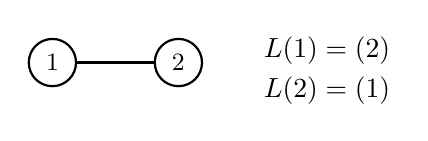
\begin{tikzpicture}[x=1.6cm]
  \node[vtx] (u) at (0,0) {1};
  \node[vtx] (v) at (1,0) {2};
  \draw[gedge] (u)--(v);
  \node[anchor=west] at (1.6,0.15) {$\Lst(1)=(2)$};
  \node[anchor=west] at (1.6,-0.35) {$\Lst(2)=(1)$};
\end{tikzpicture}
\end{center}

\begin{itemize}
  \item \textsc{Inc} requires $\Lst(1)\lex\Lst(2)$, i.e.\ $(2)\lex(1)$: \textbf{\color{red}false}.
  \item \textsc{Dec} requires $\Lst(1)\succeq\Lst(2)$, i.e.\ $(2)\succeq(1)$: \textbf{\color{teal}true}.
\end{itemize}
So under \textsc{Inc} the only non-empty graph on two vertices is lost. The solver finds
$1$ graph (the empty one) instead of $2$.
\end{example}

The reason is simple: \emph{a vertex is never its own neighbor}. Vertex $1$ cannot list
the label $1$, so its list starts with a label $\ge2$, while vertex $2$ lists $1$. The smallest
label forces vertex~1 to have the \emph{larger} list, which is exactly what \textsc{Inc}
forbids and \textsc{Dec} asks for.

\subsection{The same phenomenon for $n=3$}

\begin{example}[One edge plus an isolated vertex]\label{ex:inc3}
Let $G$ be one edge and one isolated vertex ($n=3$, two slots per list). The isolated vertex
can receive label $1$, $2$ or $3$, which gives the three labellings:

\begin{center}
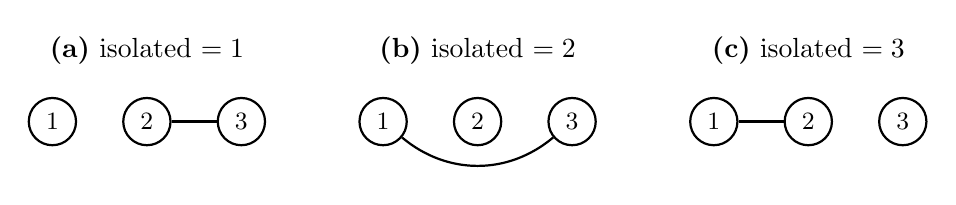
\begin{tikzpicture}[x=1.2cm]
  \node at (1,0.9) {\textbf{(a)} isolated $=1$};
  \node[vtx] (a1) at (0,0) {1};
  \node[vtx] (a2) at (1,0) {2};
  \node[vtx] (a3) at (2,0) {3};
  \draw[gedge] (a2)--(a3);
  \begin{scope}[xshift=4.2cm]
  \node at (1,0.9) {\textbf{(b)} isolated $=2$};
  \node[vtx] (b1) at (0,0) {1};
  \node[vtx] (b2) at (1,0) {2};
  \node[vtx] (b3) at (2,0) {3};
  \draw[gedge] (b1) to[bend right=40] (b3);
  \end{scope}
  \begin{scope}[xshift=8.4cm]
  \node at (1,0.9) {\textbf{(c)} isolated $=3$};
  \node[vtx] (c1) at (0,0) {1};
  \node[vtx] (c2) at (1,0) {2};
  \node[vtx] (c3) at (2,0) {3};
  \draw[gedge] (c1)--(c2);
  \end{scope}
\end{tikzpicture}
\end{center}

\begin{center}
\begin{tabular}{c ccc cc}
\toprule
labelling & $\Lst(1)$ & $\Lst(2)$ & $\Lst(3)$ & \textsc{Inc} & \textsc{Dec}\\
\midrule
(a) & $(0,0)$ & $(0,3)$ & $(0,2)$ & {\color{red}no: $\Lst(2)\succ\Lst(3)$} & {\color{red}no}\\
(b) & $(0,3)$ & $(0,0)$ & $(0,1)$ & {\color{red}no: $\Lst(1)\succ\Lst(2)$} & {\color{red}no}\\
(c) & $(0,2)$ & $(0,1)$ & $(0,0)$ & {\color{red}no: $\Lst(1)\succ\Lst(2)$} & {\color{teal}yes}\\
\bottomrule
\end{tabular}
\end{center}

All three labellings violate \textsc{Inc}, so the shape is lost; labelling (c) satisfies
\textsc{Dec}. In (a), the isolated vertex correctly gets the smallest list, but then the two
endpoints $2,3$ list each other, and again the vertex with the smaller label ($2$) lists
the larger label ($3$). This is the $K_2$ counterexample placed on labels $\{2,3\}$.
\end{example}

The complete picture for $n=3$ (all $2^3=8$ labelled graphs, $4$ shapes) is:

\begin{center}
\begin{tabular}{l l c c}
\toprule
edges & lists $\Lst(1),\Lst(2),\Lst(3)$ & \textsc{Inc} & \textsc{Dec}\\
\midrule
none            & $(0,0),(0,0),(0,0)$ & yes & yes\\
$12$            & $(0,2),(0,1),(0,0)$ &     & yes\\
$13$            & $(0,3),(0,0),(0,1)$ &     &    \\
$23$            & $(0,0),(0,3),(0,2)$ &     &    \\
$12,13$         & $(2,3),(0,1),(0,1)$ &     & yes\\
$12,23$         & $(0,2),(1,3),(0,2)$ &     &    \\
$13,23$         & $(0,3),(0,3),(1,2)$ & yes &    \\
$12,13,23$      & $(2,3),(1,3),(1,2)$ &     & yes\\
\midrule
shapes found (of 4) & & 2 & 4\\
\bottomrule
\end{tabular}
\end{center}

\textsc{Inc} keeps only the empty graph and the path; it loses the single edge and the
triangle $K_3$. \textsc{Dec} keeps exactly one labelling of each of the four shapes.

\subsection{Regular graphs: \textsc{Inc} finds nothing}

The triangle above already shows that \textsc{Inc} fails on regular graphs: $K_3$ has the single
labelling $(2,3),(1,3),(1,2)$, which is decreasing and not increasing. This is general:

\begin{lemma}\label{lem:incregular}
For $d\ge 1$, no $d$-regular graph satisfies \textsc{Inc}.
\end{lemma}

\begin{proof}
All lists have the same $p=n-1-d$ leading zeros; position $p+1$ holds the smallest neighbor.
Vertex $1$ is not its own neighbor, so $\Lst(1)_{p+1}\ge 2$. For every $j$,
$\Lst(j)\succeq\Lst(1)$ with equal zero prefixes gives $\Lst(j)_{p+1}\ge\Lst(1)_{p+1}\ge 2$:
no vertex has $1$ as its smallest neighbor, hence (lists are sorted) no vertex is adjacent to
$1$, contradicting $\deg(1)=d\ge1$.
\end{proof}

\subsection{Why the proof of Theorem~\ref{thm:main} breaks for \textsc{Inc}}

By Lemma~\ref{lem:bridge}, \textsc{Inc} requires non-decreasing degrees and, inside each degree
group, non-\emph{increasing} full rows. The analogue of Lemma~\ref{lem:reduced} for $\succeq$
is false: in Case~2 ($i$ adjacent to $j$) column $i$ of the full rows always reads $(0,1)$, so
$A[i]\slex A[j]$ regardless of the reduced comparison (Remark~\ref{rem:diag}). For $K_2$:
$A[1]=(0,1)\slex(1,0)=A[2]$ for every labelling. In list terms, row~$1$ must be the smallest
list but can never contain the smallest label~$1$, and row~$n$ must be the largest but can
never contain the largest label~$n$.

%=====================================================================
\section{Interaction with the connectivity constraint}
%=====================================================================

The upper off-diagonal connectivity constraint of the neighbors model requires
$\Lst(i)_{n-1}>i$ for every $i<n$ (the largest neighbor of $i$ has a larger label).
Theorem~\ref{thm:main} says nothing about \textsc{Dec} combined with this constraint, and in
fact they conflict: \textsc{Dec} pushes the last rows towards small labels, whereas the
connectivity constraint forces, e.g., vertex $n-1$ to be adjacent to $n$. Experimentally the
combination loses shapes (Table~\ref{tab:exp}). Soundness of \textsc{Dec} therefore holds for
enumeration \emph{without} the connectivity constraint; connected graphs can still be obtained
by filtering, or by keeping OptRevLex on the 0/1 rows, which is compatible with it.

%=====================================================================
\section{Experimental confirmation}\label{sec:exp}
%=====================================================================

The constraints were posted in IBM CP~Optimizer on the padded neighbor lists (\textsc{Dec} as
\texttt{lexicographic(M[j], M[i])} for $i<j$; consecutive pairs suffice by transitivity), all
solutions were enumerated, and the number of distinct shapes among them was computed and
compared with the known number of shapes (OEIS A000088, A001349, A005638, A033483).
The individual steps of the proof (Lemma~\ref{lem:bridge}(b) and the fact that $G^\ast$
satisfies \textsc{Dec}) were also checked exhaustively on every graph with $n\le6$.

\begin{table}[ht]
\centering
\caption{Solutions / distinct shapes found. A shape count below the known value means shapes
are lost.}
\label{tab:exp}
\begin{tabular}{l r rrr r}
\toprule
instance & known shapes & \textsc{Dec} & \textsc{Inc} & OptRevLex on rows & \textsc{Dec}+conn.\\
\midrule
all graphs, $n=2$ & 2    & 2 / 2        & 1 / 1       & 2 / 2       & -- \\
all graphs, $n=3$ & 4    & 4 / 4        & 2 / 2       & --          & -- \\
all graphs, $n=4$ & 11   & 11 / 11      & 4 / 4       & 11 / 11     & -- \\
all graphs, $n=5$ & 34   & 39 / 34      & 11 / 11     & 43 / 34     & -- \\
all graphs, $n=6$ & 156  & 209 / 156    & 51 / 50     & 276 / 156   & -- \\
all graphs, $n=7$ & 1044 & 1813 / 1044  & 418 / 373   & 3158 / 1044 & -- \\
connected, $n=7$  & 853  & --           & --          & 2796 / 853  & 48 / 24 \\
$3$-regular, $n=6$ & 2   & 2 / 2        & 0 / 0       & 2 / 2       & -- \\
$3$-regular, $n=8$ & 6   & 23 / 6       & 0 / 0       & 15 / 6      & -- \\
$4$-regular, $n=8$ & 6   & 22 / 6       & 0 / 0       & 13 / 6      & -- \\
\bottomrule
\end{tabular}
\end{table}

\textsc{Dec} keeps every shape in all cases, as predicted by Theorem~\ref{thm:main}, and
for all graphs it produces fewer duplicate labellings than OptRevLex on the adjacency rows
(1813 vs.\ 3158 at $n=7$). \textsc{Inc} loses shapes everywhere, and $0$ solutions on every
regular instance, as predicted by Lemma~\ref{lem:incregular}.

%=====================================================================
\section{Relation to the literature}
%=====================================================================

Lemmas~\ref{lem:reduced} and~\ref{lem:swap} are the argument used by Codish, Miller, Prosser
and Stuckey~\cite{codish13,codish19} to prove soundness of the reduced row order
(OptLex) and of the row ordering of Miller and Prosser. The general principle that the
lexicographically smallest member of a symmetry class satisfies such constraints goes back to
lex-leader constraints~\cite{crawford96} and orderly generation~\cite{read78}.
The contributions here are:
\begin{enumerate}
  \item the bridge Lemma~\ref{lem:bridge}, which translates the order on padded neighbor lists
  into ``degree first, then the reversed adjacency-row order'';
  \item the observation that the swap argument still works when the minimum is taken only over
  labellings with non-increasing degrees, because swapping two vertices of equal degree stays
  inside that set.
\end{enumerate}

\begin{thebibliography}{9}
\bibitem{codish13}
M.~Codish, A.~Miller, P.~Prosser, P.~J.~Stuckey.
\newblock Breaking symmetries in graph representation.
\newblock In \emph{Proc.\ IJCAI 2013}, pp.~510--516.

\bibitem{codish19}
M.~Codish, A.~Miller, P.~Prosser, P.~J.~Stuckey.
\newblock Constraints for symmetry breaking in graph representation.
\newblock \emph{Constraints}, 24(1):1--24, 2019.

\bibitem{crawford96}
J.~Crawford, M.~Ginsberg, E.~Luks, A.~Roy.
\newblock Symmetry-breaking predicates for search problems.
\newblock In \emph{Proc.\ KR 1996}, pp.~148--159.

\bibitem{read78}
R.~C.~Read.
\newblock Every one a winner, or how to avoid isomorphism search when cataloguing
combinatorial configurations.
\newblock \emph{Annals of Discrete Mathematics}, 2:107--120, 1978.
\end{thebibliography}

\end{document}
